\documentclass[../Main.tex]{subfiles}
\begin{document}

    This chapter describes the background necessary for our work. At the beginning, we outline the core concepts of machine learning and neural networks. The key elements of image style transfer are briefly explained afterwards.

\subsection{Machine Learning} 
    Machine Learning (ML) is the 'field of study that gives computers the capability to learn without being explicitly programmed' \cite{Samuel1959SomeSI}. Technically, machine learning is an approach to data science and data analysis that involves adapting and building special models, which allow computer programs to learn through experience. It is based on many other fields such as: linear algebra, calculus, statistics, probability or graph theory. ML models are constructed and improved by algorithms which goal is to make the most accurate possible prediction.
    
    There are various ML concepts and architectures, but one can highlight three parts included in most common designs:
    \begin{itemize}
        \item Model - the part which makes predictions
        \item Parameters - the factors used by the \textbf{model} to make decisions
        \item Learner - the part that adjusts the \textbf{parameters}
    \end{itemize}
    Machine Learning works by gathering the data (where the quality of data determines the future quality of model), processing them to ensure consistence and relevance, followed by splitting them to different sets (usually: training and test sets). Next, the chosen algorithm and techniques try to build the model which is evaluated and upgraded several times to reach the appropriate level of prediction accuracy \cite{deepai}. ML model needs well-prepared data to work properly. A prepared batch of data usually includes label describing its type. It enables algorithm to distinguish the batches and learn about their specific features. 

    One way that we can classify the tasks that machine learning algorithms solve is by the amount of labeled data and the generated feedback. In the first type, the significant amount of labeled data is provided and the model generates some output. This paradigm is called \textbf{supervised learning}. In another paradigm, no labeled data is provided, no feedback generated - it is  \textbf{unsupervised learning}. Lastly, the \textbf{reinforcement learning}, rather different from the previous ones, take suitable action to maximize reward in a particular situation. The three main paradigms of ML are depicted in Figure \ref{fig:ML-paradigms}. \\
    \begin{figure}[h]
        \centering
        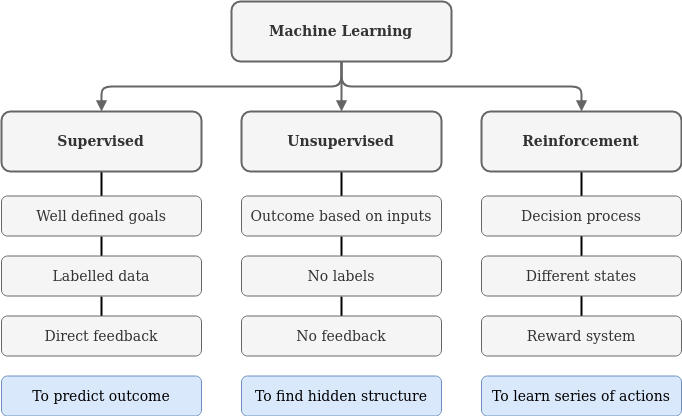
\includegraphics[width=0.7\textwidth]{ML-paradigms}
        \caption{Machine Learning paradigms}
        \label{fig:ML-paradigms}
    \end{figure}

    There are a whole bunch of different applications to which machine learning methods can be implemented. The most popular ones \cite{MLgoogle} incl.: Natural Language Processing, Classification Problems, Learning Associations, Pattern Recognition and Image Processing which is the one we focus on in this paper.


\subsection{Neural Networks}
    \subsubsection{Overview}
    The neural network is a concept and technique for building a computer program that learns from data and which is based very loosely on how the human brain works. More precisely, it is a collection of artificial \textbf{neurons} which are connected and allowed to send messages to each other. When this collection is asked to solve a problem, it attempts to do so over and over, each time strengthening the connections that lead to successful solution and reduce those leading to the wrong one \cite{tfplayground}.
    
    Technically, neural networks are \textbf{weighted graphs}. They consist of an ordered set of layers, where every layer is a group of neurons (nodes). The first layer of the neural network is called the \textbf{input layer}, and the last one is called the \textbf{output layer}. The layers in between are named \textbf{hidden layers}. Nodes belonging to one layer are connected to the nodes in the following and/or the previous layers. These connections are weighted edges. \\ 
    \begin{figure}[h!]
        \centering
        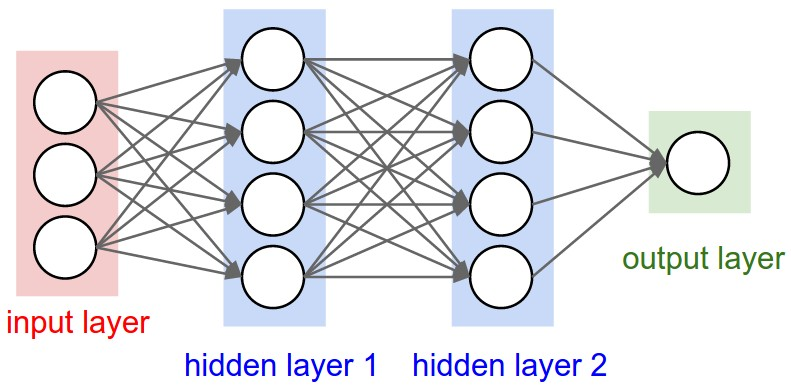
\includegraphics[width=0.7\textwidth]{cnn-network.jpeg}
        \caption{Neural network layers}
        \label{fig:nn-scheme}
    \end{figure}

    Given an input, each node produces an output (a number) which is calculated by the \textbf{activation function}. This output is then passed to the subsequently connected nodes, which calculate the next outputs. By calculating layer outputs consecutively, we calculate the output of the final layer, which is the one we need.
    
    \subsubsection{Deep Neural Networks}
    Deep neural network is simply a feedforward network with many hidden layers. 
    There is no definite answer to the question of how many layers does a network need to be qualified as deep, but usually having two or more hidden layers counts as deep. In contrast, a network with only a single hidden layer is conventionally called "shallow" \cite{Goodfellow-et-al-2016}.
    
    \subsubsection{Relationships}
    The variety of terms in the field of AI/ML may be confusing. Especially, the relations between major concepts described in this paper. Diagram presented on Figure \ref{fig:AI-ML-Scheme} tries to clarify it.
    \begin{figure}[h!]
        \centering
        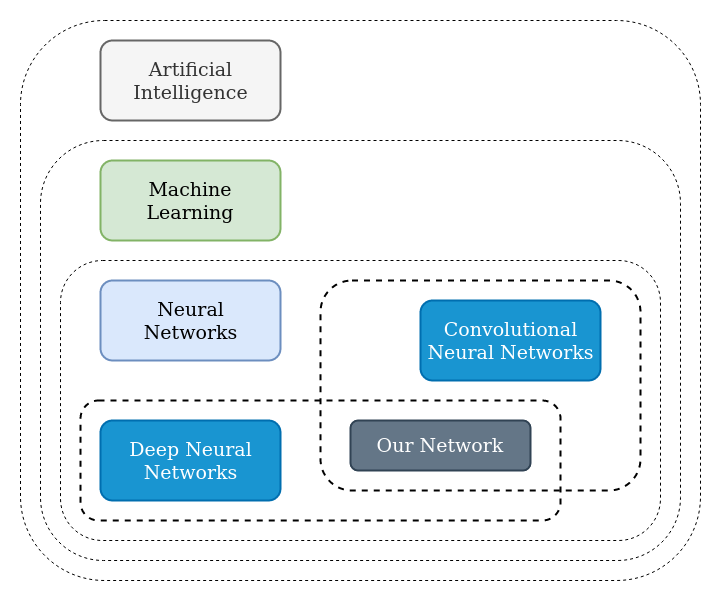
\includegraphics[width=0.7\textwidth]{AI-ML-Scheme.png}
        \caption{The relationship between main fields}
        \label{fig:AI-ML-Scheme}
    \end{figure}

\subsection{Convolutional Neural Networks}

    \subsubsection{Definition}
    \textbf{Convolution Neural Networks (CNN)} are specialized types of networks. The \textbf{convolution} itself is a specific kind of linear operation. Convolutional networks are simply neural networks that use convolution in place of general matrix multiplication in at least one of their layers \cite{Goodfellow-et-al-2016}.  CNN is well adapted for the processing of images, but the same concept also fits other fields, like audio or video. 
    Compared to the 'standard' feed-forward neural network with a similarly-sized layer, CNN could have fewer connections and parameters. Therefore it is easier to train, while its theoretically-best performance is going to be only slightly worse \cite{krizhevsky-imagenet}.
        
    \subsubsection{CNN Layers}
    The architecture of a CNN is designed to take advantage of the two-dimensional structure of an input image. Convolutional network is comprised of one or more convolutional layers followed often by subsampling step (pooling) and then by one or more fully connected layers - just as in a standard multi-layer network \cite{dlstanford}. The most common CNN layers listed below are normally placed where the hidden layers are depicted on Figure \ref{fig:nn-scheme}. 
    \begin{itemize}
        \item The \textbf{convolution layer} has to extract features from the input. It computes a dot product between neuron weights and a small region it is connected to in the input volume.
    \begin{figure}[h!]
        \centering
        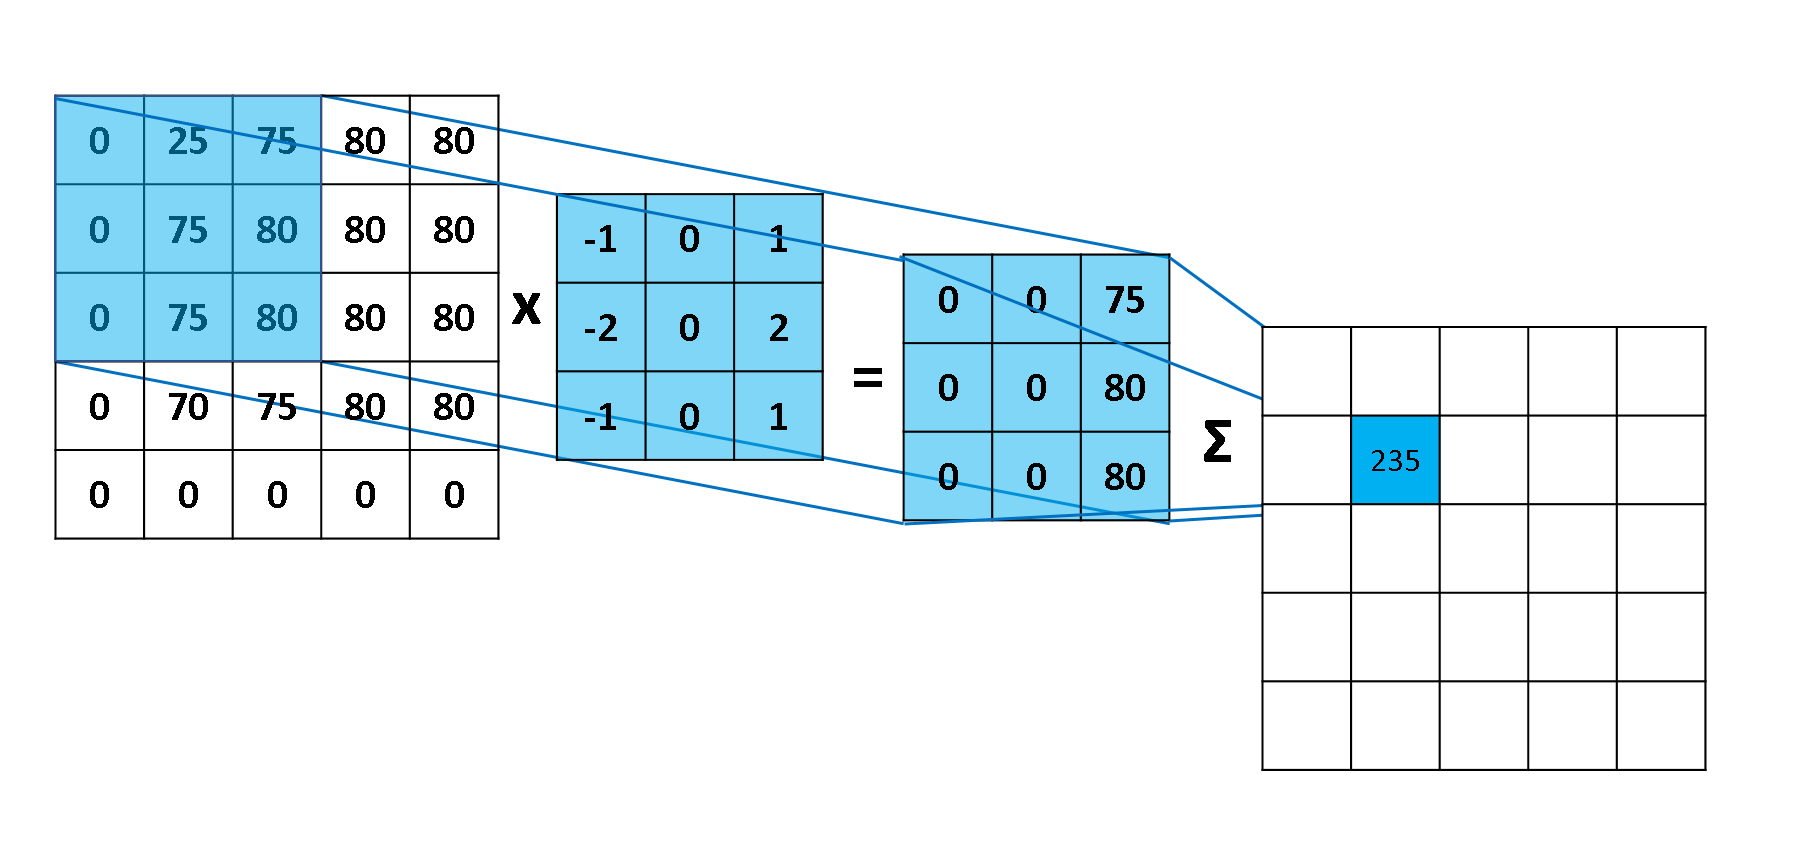
\includegraphics[width=0.5\textwidth]{cnn-convolution.png}
        \caption{Convolution with 3x3 filter}
        \label{fig:cnn-convolution}
    \end{figure}
    
        \item The \textbf{pooling layer} reduces the spatial size of these feature maps. Sometimes, the input image is a big one (and therefore time-consuming, especially if you have a large input set) or there are sparse data. In these cases, the objective of the Pooling Layers is to reduce the spatial dimension of the input matrix. A pooling layer is applied after one or multiple convolution layers.
    \begin{figure}[h!]
        \centering
        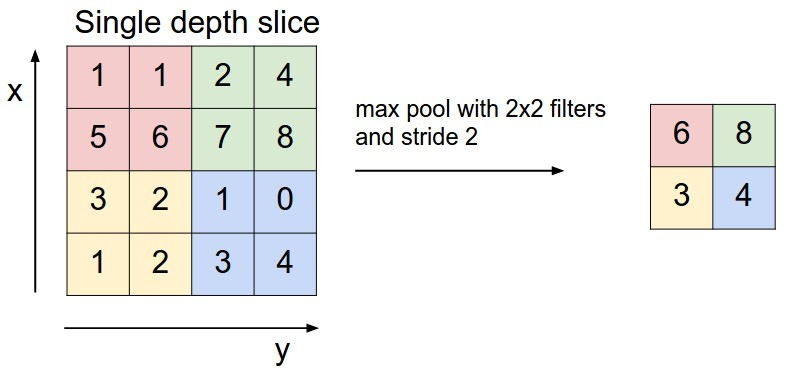
\includegraphics[width=0.5\textwidth]{cnn-pooling.jpeg}
        \caption{Process of max-pooling}
        \label{fig:cnn-pooling}
    \end{figure}
    
        \item The last one - \textbf{fully connected layer} - performs the high-level reasoning and produces the final output. Neurons in a fully connected layer have connections to \textbf{all} neurons in the previous layer.
    \end{itemize}

    \subsubsection{Activation}
    The activation function is attached to each neuron in the network, and determines whether it should be activated or not. Based on whether each neuron input is relevant for the model prediction. Activation functions also helps to normalize the output of each neuron to some range (generally between 1 and 0 or 1 and -1) \cite{missinglink}. 

    Since activation function is calculated across thousands or even millions of neurons for each data sample, it must be computationally efficient. One of the the most used one (also in our network) is \textbf{Rectified Linear Unit (ReLU)}. It applies an element-wise function, such as the max(0,x) - thresholding at zero - to either activate or deactivate each single neuron.

    \subsubsection{Loss}
    To get know if the result of operations performed in a neural network is correct (or not), we need a function that allows solutions to be ranked and compared. This is known as the \textbf{loss function}. It reduces all the various good and bad aspects of a possibly complex system down to a single number (or vector of numbers), a scalar value, which evaluates the candidate solution \cite{neuralsmithingbook}. 
    
    \subsubsection{Backpropagation}
    
    Backpropagation is an algorithm commonly used to train neural networks. When the neural network is initialized, weights are set randomly (or para-randomly). The input is loaded and then passed through the network, and it provides an output for each one neuron, given the initial weights. Backpropagation helps to adjust the weights of the neurons so that the result comes closer and closer to the known true result. It is worth to mention that backprop for a convolution operation (for both the data and the weights) is also a convolution. The description of this mechanism in our network can be found in chapter 3.

\subsection{Computer Vision}
    Computer vision is a field of computer science that tries to understand the images and videos - how they are stored, how can we manipulate and how effectively retrieve data from them. It seeks to replicate the human vision system and enable computers to \textit{think and see} the same way we do. Computer Vision plays a major role in photo correction apps and art generation but also in self-driving vehicles or robotics \cite{towardsdatascience}.
    
    Thanks to the growing popularity of AI and recent innovations in the field of Deep Learning (and Neural Networks as well), Computer Vision is developing rapidly and is able to achieve better rates in almost all areas. In many tasks, it even can surpass humans (e.g. in object detection and labeling). Since we generate and collect more data used to train and make Computer Vision better, the growth of this field will be ensured. 

\subsection{Style transfer}
    \subsubsection{Overview}
    Style transfer is a technique of extraction visual aspects from an image and blending it together with an another image content. It aims to manipulate digital pictures (or videos) and adopt the appearance or visual style. This is usually implemented by optimizing the output image to match the content statistics of the content image and the style statistics of the style reference image. These statistics are extracted from the images using a convolutional network. 
    
    The crucial part of style transfer is process of isolating the style and the content from an image. Researchers developed many approaches which enable computers to do it with high precision. We briefly introduce some techniques in next subsections. \\
    \begin{figure}[h]
        \centering
        \includegraphics[width=0.6\textwidth]{style-and-content}
        \caption{Style and content flow diagram from \cite{ulyanov2016instance}}
        \label{fig:style-and-content}
    \end{figure}
    
    \subsubsection{Example}
    One of the most common use of style transfer is creating an artificial artwork  from photo. Especially the ones produced from some famous paintings. Attached examples give an idea of this approach capabilities. \\
    \begin{figure}[h!]
        \centering
        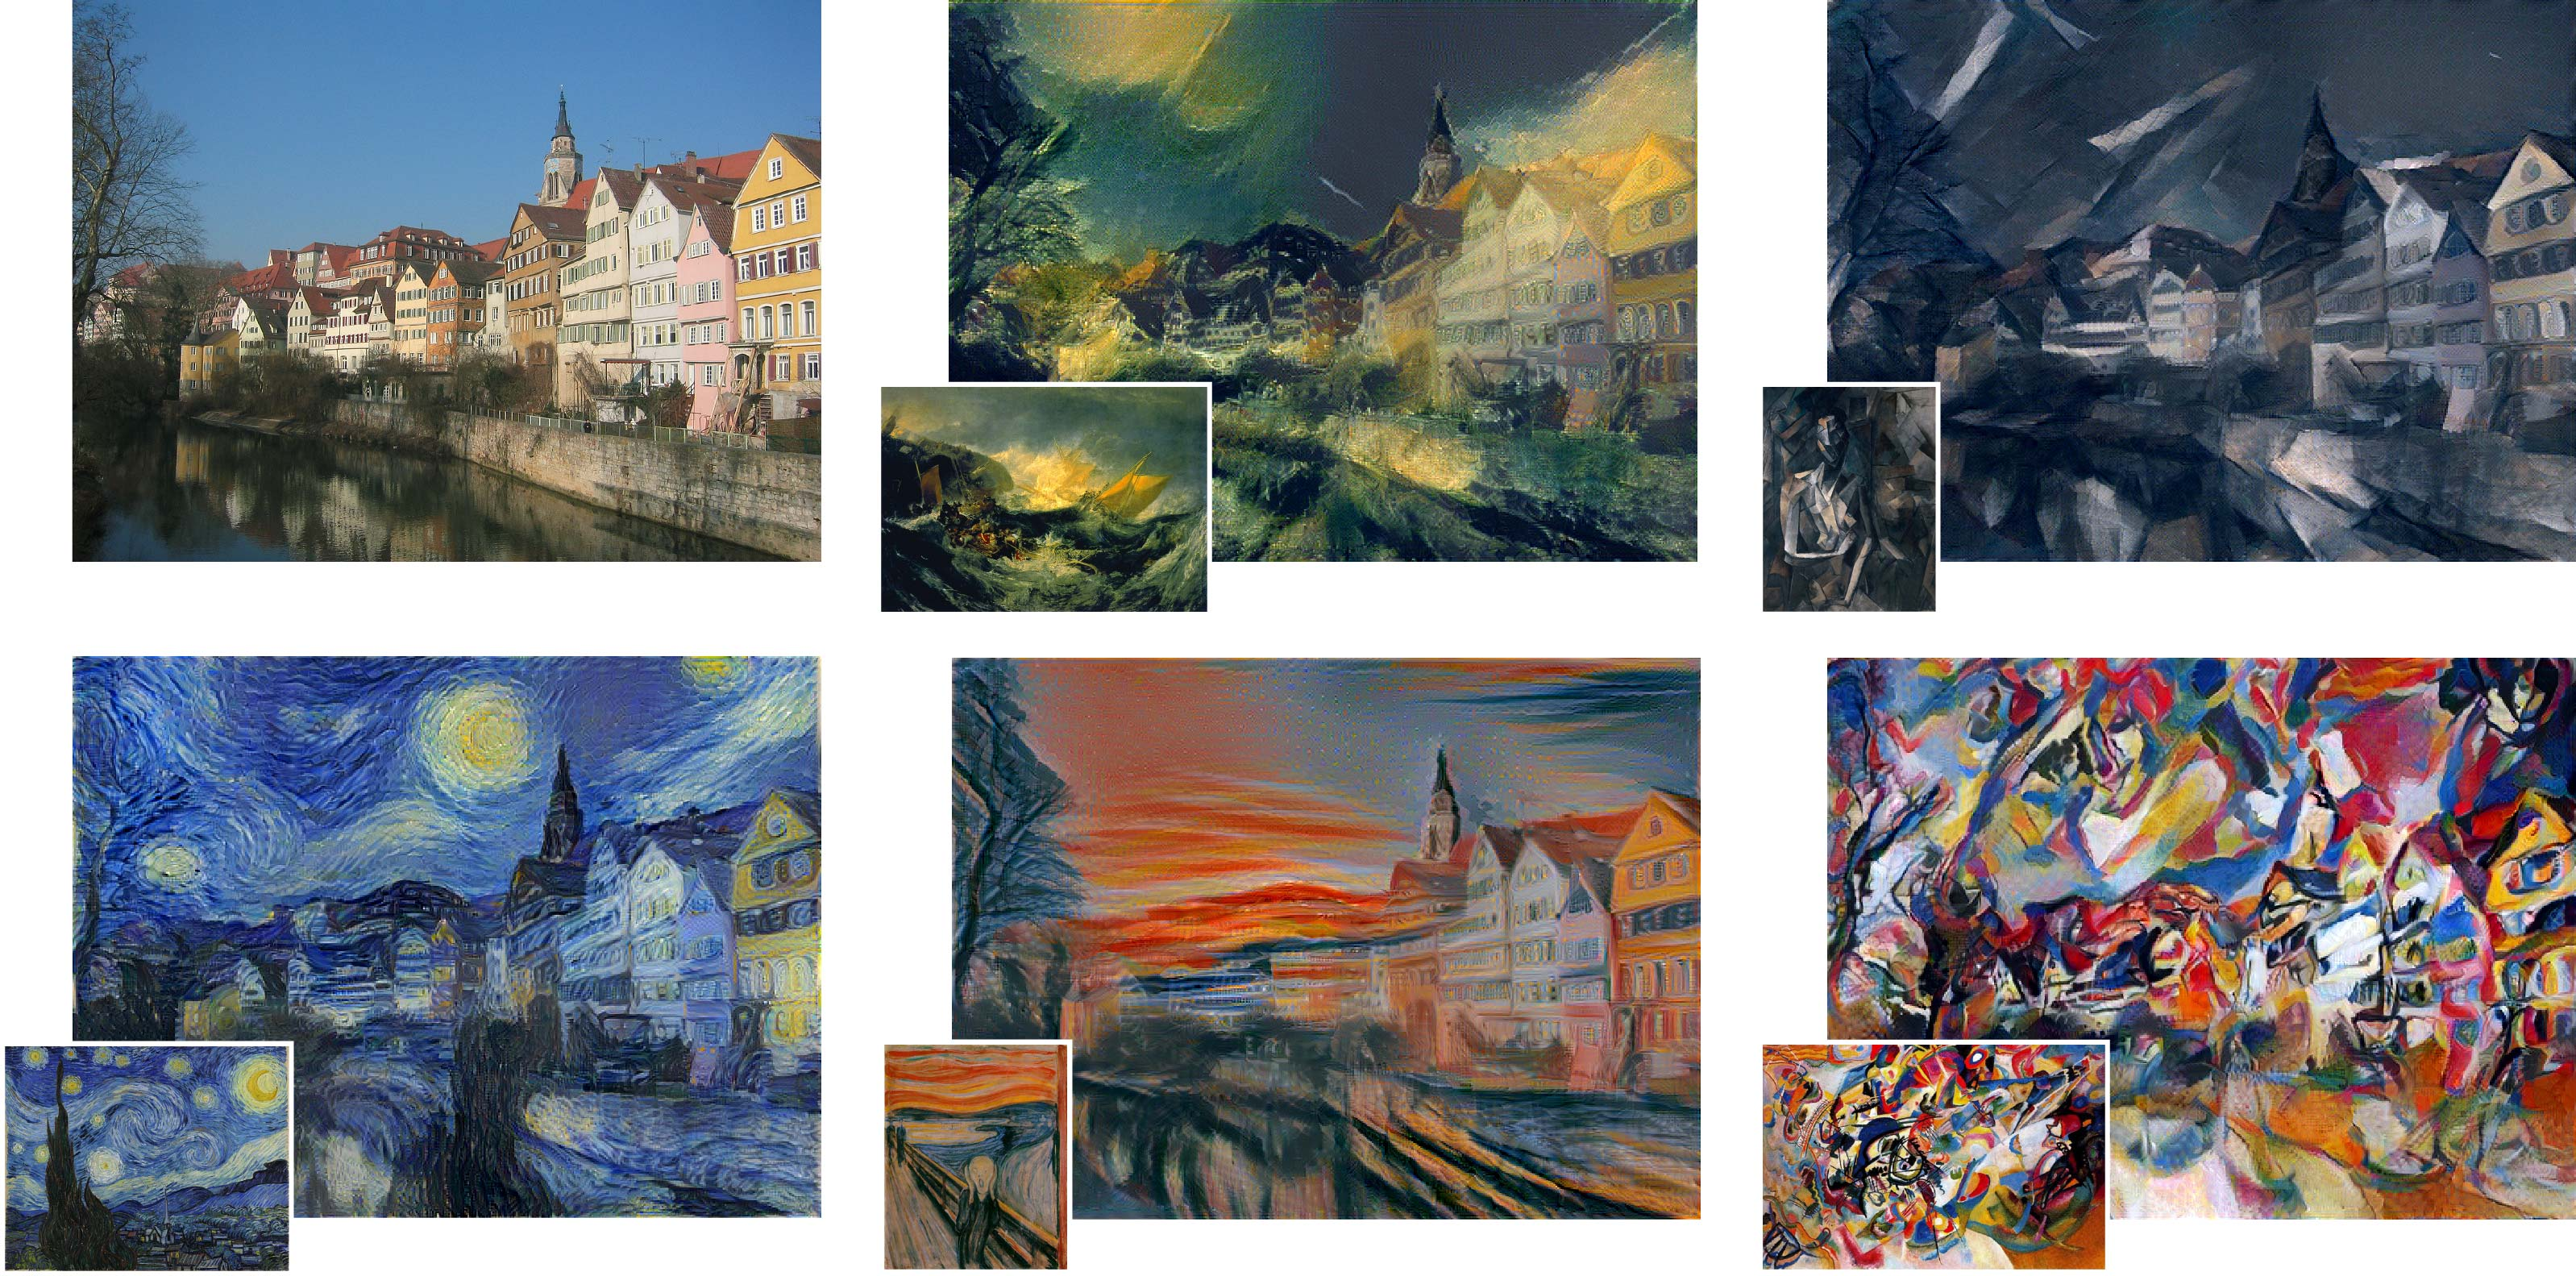
\includegraphics[width=0.7\textwidth]{ST-example-gatys.jpg}
        \caption{Picture transformed to painting-like image by \cite{gatys2015neural}}
        \label{fig:ST-example-gatys}
    \end{figure}

    \subsubsection{State of the art}
    Neural Style Transfer (NST) was first published in the paper "A Neural Algorithm of Artistic Style" by Gatys et al. \cite{gatys2015neural} and is developing rapidly gaining more and more attention. The core branches of Neural Style Transfer are presented on the Figure \ref{fig:state-of-the-art}. Since presenting every concept of NST is not the goal of this paper, we recommend to visit \href{https://github.com/ycjing/Neural-Style-Transfer-Papers}{this actively updated repository}, where one can find information about each sub-field of the Neural Style Transfer.  \\
    \begin{figure}[h!]
        \centering
        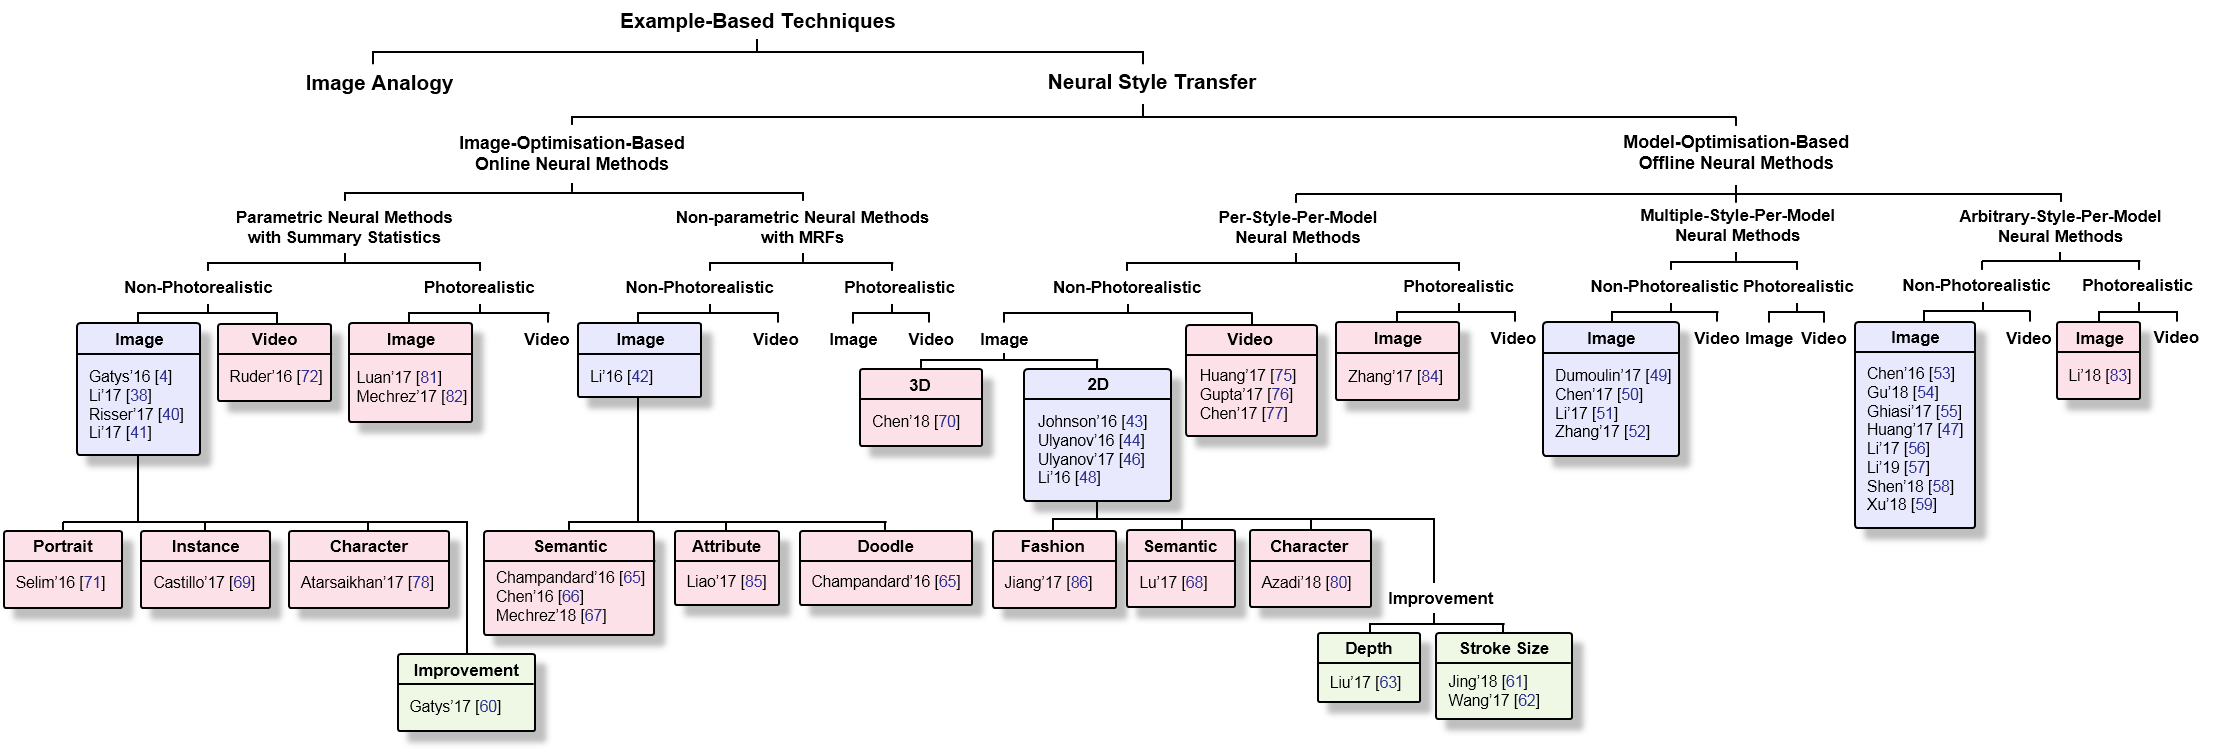
\includegraphics[width=1\textwidth]{state-of-the-art.png}
        \caption{State of the art by \cite{nstpapersrepo}}
        \label{fig:state-of-the-art}
    \end{figure}
    
    \subsubsection{Loss function in style transfer}
    In general \textbf{loss function} in NST contains two sub-losses: the content reconstruction loss and the style reconstruction loss. The idea is pretty straightforward. The first loss ensures that the activations of the higher layers are similar between the content image and the generated image. The second one makes sure that the correlation of activations in all the layers are similar between the style image and the generated image. So the differences between source and output image are the basis of the loss computing.
    The concept can be denoted as follows:
    \[L= \alpha L_{content} + \beta L_{style}\]
    where $\alpha$ and $\beta$ are hyperparameters. By controlling them one can decide how much style of source image will be preserved (and similarly - the amount of the source image content). 
    
    \cite{gatys2015neural} proved that CNN captures the content info in higher levels of the network. Whereas \cite{zeiler2013visualizing} states that if two images have the same content, the activations in their higher levels are similar. It is the core idea of many content loss calculation methods.
    Style reconstruction loss is usually more advanced topic, but plenty of approaches base on correlation between feature maps. It is also common to compute style losses at multiple levels (while content loss is computed only once).

    \subsubsection{AdaIn}
    Among many approaches to the (Artistic) Neural Style Transfer we would like to highlight the AdaIN method \cite{huang2017adain}. The authors of the Adaptive Instance Normalization aimed to speed up the computationally efficient style transform process. They pointed out that even the best methods cost a lot - either time or computing resources. Therefore are not designed for commercial use, particularly in real-time processing programs. Moreover, their method is free from restriction of pre-defined set of styles. It seemed to achieve all objectives of our project.
    In a nutshell, the approach uses the \textbf{instance normalization (IN)} - the alternative to the batch normalization, which computes the mean and standard deviation, and then normalize across each channel in each training example separately. The authors designed extension to IN which 'adjusts the mean and variance of the
    content input to match those of the style input'. It enables fast processing and full user control of the image styling.
    
    Despite the numerous advantages, AdaIN has some cons mentioned in the paper. First of all, the quality of generated image is questionable when method does not involve firstorder statistcis like variance \cite{Li2018}. Due to the three-way trade-off between the quality, user-flexibility and speed, authors accept this downside. But what is more crucial and important for our work, the speed of the algorithm run is 56 FPS for 256x256 and 15 FPS for 512×512. It is way too low on the good authors' machine architecture, especially when we are going to consider processing 1024x576 frames with speed at least 20 FPS.
    Nevertheless, we find AdaIN idea interesting and out-of-the-box. It might be that future work and experiments will enhance the possibilities and meet our expectations.

    \subsubsection{Commercial use}
    Some research projects became a base of mobile applications or web-services which can be used by everyone for any purpose:
    \begin{itemize}
        \item \href{https://deepart.io}{DeepArt} - free website where one can turn photo into artistic image
        \item \href{http://neuralstyler.com}{Neural Styler} - NeuralStyler Artificial Intelligence converting videos into art works by using styles of famous artists
        \item \href{https://www.ostagram.me/static_pages/lenta?last_days=1000&locale=en}{Ostagram} - web-service for algorithm combining the content of one image with the style of another image using CNN
        \item \href{https://prisma-ai.com}{Prisma} - photo-editing application able to create artwork from image
    \end{itemize}

    
    \subsubsection{Image Analogy - the obsolete approach}
    The alternative CNN approach which used to be popular beforehand is called \textbf{image analogy}. In brief, the algorithm wants to find an analogous image B' that relates to B in the same way as A' relates to A \cite{imageanalogy}. To transfer the style of image we need a dataset of training pairs of photo and an artwork from processed photo. The main weakness of this method is that mentioned pair barely exist in practice. An artwork is seldom based on a particular photo.


\subsection{Neural network compression}
    Latest neural networks usually have between 2 million and 50 million parameters.
    Older architectures are even heavier - full VGG16 model has as much as
    138 million parameters. In consequence models 
    are often too big for deployment on memory bounded mobile and embedded devices.
    Number of parameters strongly correlates with inference time, which in turn
    prevents real-time inference not only on embedded and mobile
    devices but even on middle-class GPUs. Overcoming these limitations 
    is very active area of research.\\
    \textbf{Specialized architectures} such as MobileNet \cite{mobilenetv1, 
    mobilenetv2, mobilenetv3} and ShuffleNet \cite{shufflenetv1,
    shufflenetv2}, replace full convolutions with bottlenecks of lighweight
    pointwise, depthwise and group convolutions in order to reduce number of 
    arithmetic operations and parameters. MobileNetV3 \cite{mobilenetv3} uses
    Neural Architecture Search to optimize the network for mobile phone CPU
    inference, while discussion in \cite{shufflenetv2} shows what aspects should
    be considered, when designing mobile architecture manually. 
    \textbf{Network pruning} aims to reduce already trained model's size by pruning away
    weights with the least impact on network's quality. \cite{zhu2017prune} show
    that for some models even up to $87.5$ weights \kamil{87.5\% of weights?} can be removed with only 
    marginally reduced performance. 
    Because networks are initialized randomly, the least
    important parameters are usually spread across whole network. Naive pruning 
    then results in sparse networks. Their storage is significantly reduced, however
    due to the fact that available linear algebra libraries are optimized for dense structures,
    their inference time does not scale as well. To overcome this, more structured
    methods of pruning were developed, among them filter pruning \cite{li2016pruning, molchanov2016pruning}
    and channel pruning \cite{he2017channel}. 
    Weight or weights set importance can be measured by various heuristics. 
    \cite{li2016pruning} prune away the filters with the smallest $\ell_1$ norm.
    This approach easily generalizes to $\ell_p$ norm.
    \cite{polyak2015} choose to prune away the filters with
    the smallest activation statistics. More direct methods formulate pruning 
    try to preserve performance metrics (e.g. low loss, high accuracy) on training set. 
    \cite{molchanov2016pruning} formulate pruning as optimization problem where
    the goal is preserving original training set loss value, that is minimizing
    $|L_{new} - L_{orig}|$. Curiously changing the goal to $L_{new} - L_{orig}$,
    that is letting the loss drop, degrades the resulting network's performance.\\
    Smaller networks can also be trained with aid of larger ones through process called
    \textbf{knowledge distillation} \cite{hinton2015distilling}. 
    The key idea is that activations of certain layers
    contain knowledge which is not present in dataset labels. For example in a network  trained for classification, the final softmax layer outputs are usually 
    interpreted as probabilities of respective classes. These probabilities might indicate that for given input x, $C_1$ is the proper class and class $C_2$ is twice as probable 
    as class $C_3$. If the network is well trained this means x is more similar to
    objects of class $C_2$, rather than $C_3$. By training a new small network to match its both
    softmax outputs with the larger trained network softmax outputs and proper labels,
    we effectively gain additional training data and ease the training.
    Almost every network inference time can also be increased by \textbf{quantization}.
    In many deep learning frameworks, computation is by default performed on
    32-bit floating point numbers. Such precision is often required during training to 
    ensure gradient numerical stability. However given that network weights have
    relatively small magnitude, in many applications it is unnecessary during inference.
    Modern GPUs enable inference in FP16 and INT8 modes. There has also been worked 
    on even lower precision inference, performed on CPUs. 
    
        
\biblio % Needed for referencing to working when compiling individual subfiles - Do not remove
\end{document}
